\chapter{Behoudsvergelijkingen langs stroomlijnen}
\label{sec:Behoudsvergelijkingen langs stroomlijnen}

%%%%%%%%%%%%%%%%%%%%%%%%%%%%%%%%%%%%%%%%%%%%%%%%%%%%%%%%%%%%%%%%%%%%%%%%%%%%%%%%%%%%%%
	\section{Inleiding}
	\label{sec:Behoudsvergelijkingen langs stroomlijnen inleiding}

%%%%%%%%%%%%%%%%%%%%%%%%%%%%%%%%%%%%%%%%%%%%%%%%%%%%%%%%%%%%%%%%%%%%%%%%%%%%%%%%%%%%%%
	\section{Bewegingsvergelijking langs de stroomlijnen}
	\label{sec:Bewegingsvergelijking langs de stroomlijnen}
De uitwerking van de bewegingsvergelijking in cartesiaanse coördinaten is niet voor de hand liggend en bied weinig inzicht. Een eenvoudig alternatief is de uitwerking in stroomlijn coördinaten. Kies hiervoor een $s$ coördinaat die de stroomlijnen volgt in de richting van de stroming. Een $n$ coördinaat vector kunnen we nu definiëren door de $\vt{s}$ vector 90$^\circ$ in tegenwijzerzin te draaien (Figuur \ref{fig:stroomlijncoordinaten}). We kunnen dan elk punt in de stroming karakteriseren door de stroomlijn die door dit punt gaat ($n$) en de afstand langs de stroomlijn tot een bepaalde referentie ($s$). De richtingen van $s$ en $n$ coördinaat zullen nu wel in elk punt van de stroming verschillen. 
\begin{figure}[htb]
	\centering
	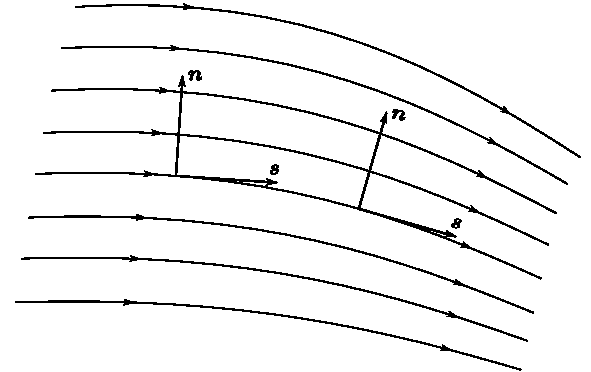
\includegraphics{fig/deeltjesvergelijkingen/Stoomlijncoordinaten}
	\caption{Voorbeeld van stroomlijncoördinaten}
	\label{fig:stroomlijncoordinaten}
\end{figure}

Beschouw nu een willekeurige stationaire niet viskeuze stroming. Kiezen we een controle volume in de stroming tussen twee stroomlijnen met lengte $\Delta s$ zoals in Figuur \ref{fig:controlevolume tussen stroomlijnen}.
\begin{figure}[htb]
	\centering
	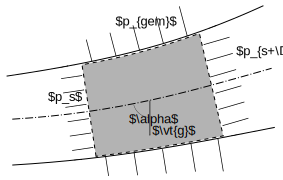
\includegraphics{fig/deeltjesvergelijkingen/Controlevolume_tussen_stroomlijnen}
	\caption{Controlevolume tussen twee stroomlijnen}
	\label{fig:controlevolume tussen stroomlijnen}
\end{figure}
Indien we de stroomlijnen dicht genoeg bij elkaar kiezen en we het controlevolume zeer kort houden zal de snelheid over de ingang en de uitgang ongeveer uniform zijn, en de stroming niet van richting veranderen. De impulsbalans in de richting van de gemiddelde stroomlijn voor dit controlevolume wordt dan:
\begin{equation}
	\left. \rho v v_{\perp} A \right|_{s+\Delta s} - \left. \rho v v_{\perp} A \right|_{s} = \left. p A \right|_{s} - \left. p A \right|_{s+\Delta s} + p_{gem} (\left. A \right|_{s+\Delta s}-\left. A \right|_{s}) -\rho g A_{gem} \Delta s \cos \alpha
	\label{eqn:impulsbalans controlevolume tussen stroomlijnen}
\end{equation}
Aangezien het controle volume langs een stroomlijn ligt staat de snelheid steeds loodrecht op het ingaande en uitgaande oppervlak. De cosinus in de laatste term kunnen we uitdrukken in functie van de verhouding van hoogteverandering $\left. z\right|_{s+\Delta s} - \left. z\right|_{s}$ tot $\Delta s$. Indien we (\ref{eqn:impulsbalans controlevolume tussen stroomlijnen}) delen door $\Delta s$ krijgen we:
\begin{equation}
	\frac{\left. \rho v v A \right|_{s+\Delta s} - \left. \rho v v A \right|_{s}}{\Delta s} = -\frac{\left. p A \right|_{s+\Delta s} - \left. p A \right|_{s}}{\Delta s} + p_{gem} \frac{\left. A \right|_{s+\Delta s}-\left. A \right|_{s}}{\Delta s} -\rho g A_{gem} \frac{\left. z\right|_{s+\Delta s} - \left. z\right|_{s}}{\Delta s}
\end{equation}
Indien we de limiet van bovenstaande uitdrukking nemen voor $\Delta s$ gaande naar $0$ zullen de gemiddelde druk en de gemiddelde oppervlakte naar respectievelijk de druk en de oppervlakte in het punt $s$ streven. We krijgen dan:
\begin{equation}
	\frac{\diff \rho v v A}{\diff s} = -\frac{\diff p A}{\diff s} + p \frac{\diff A}{\diff s} -\rho g A \frac{\diff z}{\diff s}
\end{equation}
De afgeleiden in de eerste termen in het linker en rechter lid kunnen we uitwerken via de kettingregel:
\begin{equation}
	\rho v A \frac{\diff v}{\diff s} +  v \frac{\diff \rho v A}{\diff s} = -A \frac{\diff p}{\diff s} - p\frac{\diff A}{\diff s} + p \frac{\diff A}{\diff s} -\rho g A \frac{\diff z}{\diff s}
\end{equation}
In de tweede term van het linker lid staat de afgeleide van $\rho v A$. Dit komt overeen met de afgeleide van het massadebiet naar de lengte van de stroomlijn. Aangezien de stroming stationair is, volgt uit behoud van massa dat deze term $0$ is. Na deling door de oppervlakte tussen de stroomlijnen en herschikken krijgen we:
\begin{equation}
	\rho v \frac{\diff v}{\diff s} + \frac{\diff p}{\diff s} + \rho g \frac{\diff z}{\diff s} = 0
	\label{eqn:vergelijking van Euler}
\end{equation}
Deze vergelijking staat bekend als de vergelijking van Euler. Het is de bewegingsvergelijking van een deeltje in een stationaire niet viskeuze stroming. Het is dus het analogon voor de tweede wet van Newton ($\vt{F} = m \frac{\diff \vt{v}}{\diff t}$) voor een fluïdum stroming. Uit deze vergelijking kan, zoals de naam doet vermoeden, de beweging van de verschillende deeltjes in de stroming worden geïntegreerd. Aangezien ze voortvloeit uit een krachten evenwicht stelt elke term een bepaalde kracht voor die op het beschouwde fluïdum deeltje inwerkt. In de eerste term herkennen we de versnelling of de traagheidskracht, de tweede term is afkomstig van drukkrachten en de derde term is afkomstig van de zwaartekracht. Een fluïdum deeltje zal dus enkel versnellen of vertragen indien er bepaalde krachten op inwerken.

		\subsection{Deeltjesversnelling}
Ook in een stationaire stroming (onafhankelijk van de tijd) kunnen de fluïdum deeltjes dus een versnelling ondergaan. Aangezien de snelheid niet overal in het stromingsveld constant moet zijn en een individueel deeltje zich door het stromingsveld verplaatst zal het inderdaad een versnelling ondergaan. Dit soort versnelling noemen we een convectieve versnelling. Ook andere eigenschappen van het fluïdum deeltje kunnen veranderen wanneer het deeltje zich door de stroming beweegt (vb. temperatuur, druk,...). Algemeen kunnen we dan spreken over een convectieve verandering van de stromingsgrootheden.

Wanneer de stroming niet stationair is kunnen de grootheden in de stroming ook veranderen ten gevolge van een verandering in de tijd. We spreken dan van een lokale verandering. De totale verandering van de eigenschappen van een bepaald deeltje in een stroming is dan de som van de lokale en de convectieve verandering.

De verandering van de eigenschap van een deeltje komt vaak voor in de fluïdummechanica. De totale differentiaal is een wiskundig begrip dat dit weergeeft. In carthesiaanse coördinaten wordt dit:
\begin{equation}
	\frac{\subsdiff}{\subsdiff t} = \frac{\partial}{\partial t} + v_x \frac{\partial}{\partial x} + v_y \frac{\partial}{\partial y} + v_z \frac{\partial}{\partial z}
\end{equation}
Hierin is de eerste term de lokale verandering, de overige termen vormen de convectieve verandering. De totale differentiaal is een manier om de verandering van de eigenschappen van een specifiek deeltje (dat zich op een bepaald tijdstip op een bepaalde positie bevindt) te relateren aan informatie uit een veld voorstelling (Euleriaanse voorstelling).

Met behulp van de deeltjesversnelling kunnen de vergelijking van Euler intuïtief uitbreiden naar niet stationaire stromingen. We doen dit door de convectieve versnelling in de vergelijking van Euler (\ref{eqn:vergelijking van Euler}) te vervangen door de deeltjesversnelling. In vector notatie wordt dit:
\begin{equation}
	\rho \frac{\subsdiff \vt{v}}{\subsdiff t} = -\nabla p + \rho \vt{g}
\end{equation}

\begin{voorbeeld}
	Bepaal voor het stationair snelheidsveld in een horizontaal vlak uit figuur \ref{fig:snelheidsveld} de deeltjesversnelling en het drukveld indien de stroming zich niet viskeus gedraagt. Het snelheidsveld wordt gegeven door:
	\begin{align*}
		v_x = -A x \\
		v_y = A y
	\end{align*}
	
	Voor een twee dimensionale stroming wordt de deeltjesversnelling in $x$ en $y$ richting:
	\begin{align*}
		\frac{\subsdiff v_x}{\subsdiff t} = \frac{\partial v_x}{\partial t} + v_x \frac{\partial v_x}{\partial x} + v_y \frac{\partial v_x}{\partial y} \\
		\frac{\subsdiff v_y}{\subsdiff t} = \frac{\partial v_y}{\partial t} + v_x \frac{\partial v_y}{\partial x} + v_y \frac{\partial v_y}{\partial y}
	\end{align*}
	Aangezien de stroming stationair is vallen de eerste termen weg. De deeltjesversnelling wordt dus:
	\begin{align*}
		\frac{\subsdiff v_x}{\subsdiff t} = A^2 x \\
		\frac{\subsdiff v_y}{\subsdiff t} = A^2 y
	\end{align*}
	
	We kunnen nu de	vergelijking van Euler in de $x$ en $y$ richting uitwerken:
	\begin{align*}
		\frac{\subsdiff v_x}{\subsdiff t} = \frac{\partial p}{\partial x} \\
		\frac{\subsdiff v_y}{\subsdiff t} = \frac{\partial p}{\partial y}
	\end{align*}
	Dus:
	\begin{equation*}
		p = \frac{1}{2} A^2 \left(x^2 +y^2 \right) + C
	\end{equation*}
	De isobaren zijn dus concentrische cirkels met het hoekpunt als middelpunt.
	\begin{center}
		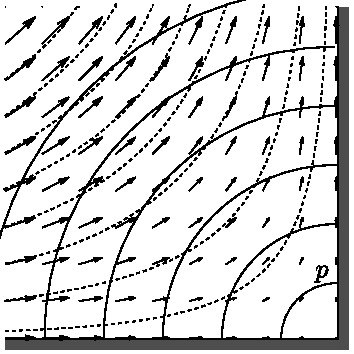
\includegraphics{fig/deeltjesvergelijkingen/Snelheidsveld_en_drukveld}
	\end{center}
\end{voorbeeld}
%%%%%%%%%%%%%%%%%%%%%%%%%%%%%%%%%%%%%%%%%%%%%%%%%%%%%%%%%%%%%%%%%%%%%%%%%%%%%%%%%%%%%%
	\section{Integratie van de bewegingsvergelijking}
	\label{sec:Integratie van de bewegingsvergelijking}
Indien we in een stroming de stroomlijnen kennen kunnen we de bewegingsvergelijking (\ref{eqn:vergelijking van Euler}) integreren. Langs een stroomlijn wordt dit:
\begin{equation}
	\int \rho v \frac{\diff v}{\diff s} \diff s + \int \frac{\diff p}{\diff s} \diff s + \int \rho g \frac{\diff z}{\diff s}  \diff s = Cst
\end{equation}
Indien de dichtheid constant is langs de stroomlijn kunnen we de integralen verder uitwerken tot:
\begin{equation}
	\frac{1}{2} \rho v^2 + p + \rho g z = \text{Cst}
	\label{eqn:vergelijking van Bernoulli}
\end{equation}
Deze vergelijking werd als eerste gepubliceerd door Daniel Bernoulli en werd nadien de vergelijking van Bernoulli genoemd. Ze geeft de relatie weer tussen snelheid, druk en hoogte van een deeltje dat zich verplaatst in een stationaire stroming. Met behulp van deze vergelijking kunnen we indien we de grootheden van de stroming in een bepaald punt kennen (randvoorwaarden) de grootheden in andere punten berekenen. Het is een vergelijking die zeer vaak gebruikt wordt in de fluïdummechanica, maar jammer genoeg ook vaak onterecht gebruikt wordt. Bij het gebruik van de vergelijking van bernoulli moeten we steeds controleren dat er aan de voorwaarden gebruikt tijdens de afleiding voldaan wordt. Deze voorwaarden zijn:
\begin{itemize}
	\item Stationaire stroming
	\item Niet-viskeuze stroming
	\item Evaluatie langs een stroomlijn
	\item Constante dichtheid langs de stroomlijn
\end{itemize}
	
%%%%%%%%%%%%%%%%%%%%%%%%%%%%%%%%%%%%%%%%%%%%%%%%%%%%%%%%%%%%%%%%%%%%%%%%%%%%%%%%%%%%%%
	\section{Mechanische arbeid van een deeltje}
	\label{sec:Mechanische arbeid van een deeltje}

Berekenen we de arbeid uitgeoefend door de krachten die inwerken op een deeltje in een stationaire niet viskeuze stroming terwijl het zich verplaatst van één punt naar een ander. De arbeid uitgeoefend door een kracht kunnen we berekenen als de kracht geprojecteerd in de verplaatsingsrichting maal de afgelegde weg. Beschouw een deeltje dat zich verplaatst langs een stroomlijn over een afstand $\diff s$. Uit de vergelijking van Euler (\ref{eqn:vergelijking van Euler}) zien we dat de inwerkende krachten (druk en zwaartekracht) een versnelling veroorzaken. De arbeid die op het deeltje uitgeoefend wordt door deze krachten zal dus een verandering van de kinetische energie veroorzaken:
\begin{equation}
	\int_1^2 \rho v \frac{\diff v}{\diff s} \diff s = - \int_1^2 \frac{\diff p}{\diff s} \diff s - \int_1^2 \rho g \frac{\diff y}{\diff s} \diff s
\end{equation}
Indien de dichtheid constant is kunnen we bovenstaande integralen uitwerken en na herschikking bekomen we
\begin{equation}
	\rho \frac{1}{2} (v_2^2-v_1^2) + (p_2-p_1) + \rho g (z_2-z_1) = 0
	\label{eqn:kinetische energie en arbeid}
\end{equation}
Dit is opnieuw de vergelijking van Bernoulli (\ref{eqn:vergelijking van Bernoulli}). We kunnen Bernoulli dus ook interpreteren als een vergelijking van behoud van mechanische energie. De som van kinetische energie, arbeid veroorzaakt door drukkrachten en potentiele energie van een fluïdum deeltje blijft constant, of de mechanische energie van een deeltje dat beweegt door een stationaire, niet-samendrukbare, niet-viskeuze stroming blijft constant.

%%%%%%%%%%%%%%%%%%%%%%%%%%%%%%%%%%%%%%%%%%%%%%%%%%%%%%%%%%%%%%%%%%%%%%%%%%%%%%%%%%%%%%
		\subsection{Grafische voorstelling}
De verschillende termen in de vergelijking van Bernoulli kunnen op eenvoudige wijze weergegeven worden in een diagram. Beschouw bijvoorbeeld een eenvoudige leiding met veranderlijke doorsnede en hoogte waardoor een niet-viskeuse, niet-samendrukbare stroming stroomt (Figuur \ref{fig:energiehoogte}). Binnen deze leiding is het eenvoudig een stroomlijn te tekenen waarlangs we de vergelijking van Bernoulli kunnen toepassen. De verschillende termen van (\ref{eqn:vergelijking van Bernoulli}) kunnen allen in de eenheid \unit{}{m} gezet worden door de vergelijking te delen door $\rho g$. De verschillende termen stellen nu elk een energiehoogte voor. De eenvoudigste term $z$ is de geodetische hoogte of de hoogte van de buis ten opzichte van een bepaald referentie niveau. Wanneer we hier de term $\frac{p}{\rho g}$ bij optellen bekomen we de pi\"ezometrische hoogte. Tellen we hier de term $\frac{v^2}{2 g}$ dan bij op bekomen we de energiehoogte. Voor een niet-samendrukbare stroming zonder energieverliezen moet deze volgens de vergelijking van Bernoulli constant zijn.
\begin{figure}[htb]
	\centering
	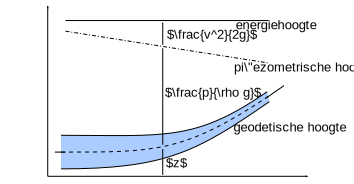
\includegraphics{fig/deeltjesvergelijkingen/Energiehoogte}
	\caption{Grafische voorstelling van de vergelijking van Bernoulli in energiehoogtes}
	\label{fig:energiehoogte}
\end{figure}

%%%%%%%%%%%%%%%%%%%%%%%%%%%%%%%%%%%%%%%%%%%%%%%%%%%%%%%%%%%%%%%%%%%%%%%%%%%%%%%%%%%%%%
	\section{Toepassingen}
Met behulp van de vergelijking van Bernoulli kunnen we een aantal interessante toestellen analyseren.
		\subsection{Pitotbuis}
Een Pitotbuis (genoemd naar Henri Pitot) is een instrument dat kan gebruikt worden voor het bepalen van de snelheid van een stroming. Het bestaat uit een buis met een opening die evenwijdig aan de snelheid in de stroming geplaatst wordt (Figuur \ref{fig:pitotbuis}) waarop een manometer aangesloten is.
\begin{figure}[htb]
	\centering
	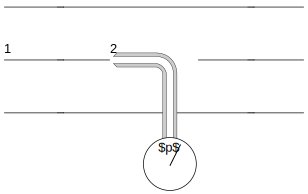
\includegraphics{fig/deeltjesvergelijkingen/Pitotbuis}
	\caption{Een pitotbuis is een stroming}
	\label{fig:pitotbuis}
\end{figure}
Schrijven we nu de vergelijking van Bernoulli uit langs de stroomlijn die in de opening van de pitotbuis uitmond. Als startpunt kiezen we een punt ver van de pitotbuis, stroomopwaarts (punt 1). Hier zal het deeltje de zelfde eigenschappen hebben als zijn omliggende deeltjes (aangezien de pitotbuis geen invloed uitoefent). De snelheid is dus de snelheid van de stroming en de druk is de heersende druk (we veronderstellen dat de hoogte constant blijft). Aangezien de pitotbuis door de drukmeter afgesloten wordt zal het fluïdum binnen in de pitotbuis stilstaan. Aan de opening van de pitotbuis zal er dus ook geen fluïdum de pitotbuis in kunnen stromen. De snelheid van de stroming in het punt 2 zal dus ook 0 zijn. Een punt waar de snelheid van de stroming daalt tot 0 of met andere woorden waar de stroming tot stilstand komt noemen we een \emph{stagnatiepunt}. De vergelijking van Bernoulli tussen punt 1 en punt 2 wordt dus:
\begin{equation}
	\frac{1}{2} \rho v_1^2 + p_1 = p_2
\end{equation}
De druk die we aflezen op de manometer is dus de druk in de vrije stroming plus de kinetische energie in de vrije stroming. We noemen dit de \emph{stagnatiedruk}. De werkelijke druk die heerst in punt 1 noemen we de \emph{statische druk}. 
\begin{eqnarray}
	p_{statisch}  &=& p \\
	p_{stagnatie} &=& p + \frac{1}{2} \rho v^2
\end{eqnarray}
Bij een niet-samendrukbare, stationaire, niet viskeuze stroming is de druk die heerst in een stagnatiepunt dus de stagnatiedruk.

Wanneer we in een leiding als in Figuur \ref{fig:energiehoogte} op verschillende plaatsen pitot buizen in de leiding plaatsen en aansluiten op een vloeistof manometers zullen de vloeistof hoogten in alle manometers ook gelijk zijn. De drukken die heersen in de verschillende manometers zijn namelijk de dynamische drukken en aangezien de manometer zich op een hoogte $z$ bevindt wordt de totale hoogte in manometer $i$:
\begin{equation}
	\frac{v_i^2}{2 g} + \frac{p_i}{\rho g} + z_i
\end{equation}
Dit is net het linkerlid van de vergelijking van Bernoulli en is dus constant.

Met behulp van een pitotbuis en een statische drukmeting kan nu de snelheid van de vrije stroming bepaald worden. Wanneer we inderdaad de statische druk van de dynamische druk aftrekken (door bijvoorbveeld het de verschildruk tussen statische en dynamische druk te meten) houden we de kinetische energie van de vrije stroming over. Wanneer nu de dichtheid van het fluïdum gekend is kunnen we de snelheid berekenen.

Een toestel dat de dynamische druk met de statische druk vergelijkt noemen we een Pitot-statisch buis (vaak wordt dit toestel ook gewoon pitotbuis genoemd). Deze toestellen vormen nog steeds de basis voor snelheidsmetingen in de luchtvaart. 

		\subsection{Venturi effect}
Het venturi effect (genomed naar Giovanni Battista Venturi) is een fenomeen dat optreed bij een lokale vernauwing in een buis (Figuur \ref{fig:venturi}).
\begin{figure}[htb]
	\centering
	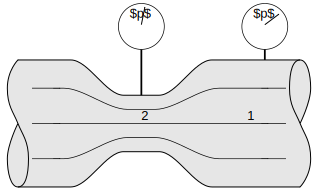
\includegraphics{fig/deeltjesvergelijkingen/Venturi}
	\caption{Een vernauwing in een buis}
	\label{fig:venturi}
\end{figure}
In de vernauwing zal volgens het behoud van massa de snelheid stijgen. Uit de vergelijking van Bernoulli weten we dat wanneer de snelheid stijgt en de hoogte constant blijft de druk zal dalen. Tussen punt $1$ en $2$ wordt dit:
\begin{equation}
	p_2 = p_1 - \rho \frac{1}{2}\left(v_2^2-v_1^2\right) = p_1 - \rho \frac{1}{2} v_1^2 \left(\frac{A_1^2}{A_2^2}-1\right)
\end{equation}
Wanneer er in punt $1$ atmosfeerdruk heerst zal er in punt $2$ dus een onderdruk heersen. Wanneer we een kanaal aansluiten op de buis in de vernauwing kunnen we dus een ander fluïdum aanzuigen door dit kanaal en mengen met de hoofd stroming. Dit principe werd vroeger gebruikt in de carburator van benzine wagens. De lucht die de cilinders in stroomt werd door een vernauwing geleid. Op deze vernauwing was een kanaal aangesloten waardoor brandstof aangezogen werd. Wanneer het luchtdebiet stijgt zal ook de onderdruk in de vernauwing stijgen en wordt er dus meer brandstof aangezogen. Dit principe is echter verdrongen door de brandstof injectie bij personenwagens sinds de jaren 90. Bij motoren wordt de carburator wel nog vaak gebruikt.

Een andere toepassing van het venturi effect is de venturi vacuüm pomp. Hier wordt de drukdaling in de vernauwing gebruikt om een vacuüm te genereren. 

%%%%%%%%%%%%%%%%%%%%%%%%%%%%%%%%%%%%%%%%%%%%%%%%%%%%%%%%%%%%%%%%%%%%%%%%%%%%%%%%%%%%%%
	\section{Energiebeschouwingen en irreversibiliteit}
	\label{sec:Energiebeschouwingen en irreversibiliteit}
In het voorgaande gedeelte bekwamen we dat de vergelijking van Bernoulli een energievergelijking is voor een niet-viskeuze, niet-samendrukbare stroming langsheen een stroomlijn. In Hoofdstuk \ref{sec:Behoudsvergelijkingen voor controlevolumes} bekwamen we echter reeds een vergelijking voor behoud van energie voor een stationair controlevolume met één instroming en één uitstroming (\ref{eqn:behoud van energie in een controlevolume met een in en uitstroming asvermogen}). Indien we deze vergelijking delen door het massadebiet bekomen we:
\begin{equation}
	(u_u + \frac{p_u}{\rho_u} + \frac{1}{2}v^2_u + g z_u) - (u_i + \frac{p_i}{\rho_i}+ \frac{1}{2}v^2_i + g z_i) = q-w_a
\end{equation}
Hierin is $q$ de toegevoegde warmte en $w_a$ de onttrokken arbeid per eenheid massa die door het controlevolume stroomt. Indien deze beiden $0$ zijn kunnen we op dezelfde wijze als in sectie (\ref{sec:Bewegingsvergelijking langs de stroomlijnen}) deze vergelijking schrijven langs een stroomlijn van een stationaire stroming:
\begin{equation}
	u + \frac{p}{\rho} + \frac{1}{2}v^2 + g z = \text{Cst}
	\label{eqn:behoud van energie lang een stroomlijn}
\end{equation}
Nu zien we dat in deze vergelijking enkel de term van de inwendige energie verschillend is met de vergelijking van Bernoulli. Aangezien de vergelijking van Bernoulli enkel geldig was voor niet viskeuze stromingen en we deze voorwaarde niet hebben bij de bovenstaande vergelijking komen we tot de conclusie dat bij niet-samendrukbare viskeuze stromingen een gedeelte van de mechanische energie zal omgezet worden in inwendige energie.

De inwendige energie van een fluïdum komt tot uiting als zijn temperatuur. De meeste vloeistoffen hebben echter zo'n grote warmtecapaciteit dat de temperatuursverandering ten gevolge van een verlies van mechanische energie niet merkbaar is. Neem als voorbeeld een stroming van water die ten gevolge van energieverliezen een drukverandering van \unit{1}{bar} ondergaat. Dit komt overeen met een mechanisch energieverlies van ongeveer \unit{100}{J/kg}. De warmtecapaciteit van water bij 20\degC\ is \unit{4180}{J/kg K}. De drukverandering komt dus overeen met een temperatuursverandering van 0.024\degC. Deze verandering is zeer klein en bijna niet meetbaar.

Uit de thermodynamica weten we dat wanneer de dichtheid constant blijft een stijging van inwendige energie gepaard gaat met een stijging van entropie ($T\diff s = \diff u + p \diff v$). Aangezien er geen warmte toe of afgevoerd wordt kan deze stijging enkelveroorzaakt worden door irreversibiliteiten. Dus bij een niet-samendrukbare stroming is de omzetting van mechanische energie naar inwendige energie irreversibel.

%%%%%%%%%%%%%%%%%%%%%%%%%%%%%%%%%%%%%%%%%%%%%%%%%%%%%%%%%%%%%%%%%%%%%%%%%%%%%
	\section{Bewegingsvergelijking loodrecht op de stromingsrichting}
Ook in de richting loodrecht op de stroomlijnen kunnen we het behoud van impuls toepassen. Stellen we voor de eenvoud dat de stroming twee-dimensionaal is (in dit geval is de richting loodrecht op de stroomlijnen eenduidig bepaald). Beschouwen we hierin een  infinitesimaal klein controle volume tussen twee stroomlijnen met diepte $\Delta z$. Bij verwaarlozing van de zwaartekracht wordt de vergelijking van behoud van impuls:
\begin{equation}
	\left.\rho v_{\parallel} v_{\perp} \Delta n \Delta z \right|_{s+\Delta s}-
	\left.\rho v_{\parallel} v_{\perp} \Delta n \Delta z \right|_{s} = 
	\left. p \Delta s \Delta z \right|_{n} - \left. p \Delta s \Delta z \right|_{n+\Delta n} 
\end{equation}
Waarin $v_{\parallel}$ de component van de snelheid evenwijdig met de rand van het controlevolume voorstelt.
De krachten die in deze richting op het controle volume inwerken zijn de drukkrachten aan weerszijden.
We kunnen het controle volume steeds zo kiezen dat de snelheid parallel aan de ingang van het controle volume $0$ is. Wanneer we de kromtestraal $R$ van de gemiddelde stroomlijn kennen, kunnen we de parallelle snelheid aan de uitgang schrijven als:
\begin{equation}
	v_{\parallel}|_{s+\Delta s} = \frac{v}{R} \Delta s
\end{equation}
Hierin gebruiken we de conventie dat $R$ steeds groter dan 0 is en dat $\vt{n}$ van het middelpunt van de aanliggende cirkel weg staat. Na deling door $\Delta s$,  $\Delta n$ en $\Delta z$ en het nemen van de limiet voor $\Delta n$ gaande naar nul wordt de impulsbalans:
\begin{equation}
	\rho \frac{v^2}{R} = \frac{\partial p}{\partial n}
\end{equation}
Hierin zien we dat er enkel een variatie in druk loodrecht op de stroomlijnen kan bestaan indien de stroomlijnen een eindige kromtestraal hebben. Indien de stroomlijnen rechten zijn, is de kromtestraal oneindig en dus de drukverandering loodrecht op de stroomlijnen $0$.
	
%%%%%%%%%%%%%%%%%%%%%%%%%%%%%%%%%%%%%%%%%%%%%%%%%%%%%%%%%%%%%%%%%%%%%%%%%%%%%
	\section{Navier-Stokes vergelijkingen}
Wanneer de viscositeit wel invloed heeft op de stroming dienen we deze invloed in de bewegingsvergelijkingen te verwerken. Dit werd voor het eerst gedaan door  Claude-Louis Navier en  George Stokes. De resulterende bewegingsvergelijkingen werden dan ook naar hun vernoemd. De afleiding van deze vergelijkingen valt buiten het bereik van deze cursus. We zullen de resultaten echter wel kort bespreken.

De Navier-Stokes vergelijkingen kunnen zeer compact geschreven worden met behulp van enkele vector operators. Voor een niet-samendrukbare stroming van een Newtoniaanse vloeistof geeft dit:
\begin{equation}
	\rho \frac{\subsdiff \vt{v}}{\subsdiff t} = -\nabla p + \rho \vt{g} + \mu \nabla^2 \vt{v}
	\label{eqn:navier-stokes vergelijkingen}
\end{equation}
Geprojecteerd op de $x$-richting van een carthesiaans assenstelsel geeft dit:
\begin{equation}
	\rho \left(\frac{\partial v_x}{\partial t} + v_x \frac{\partial v_x}{\partial x} + v_y \frac{\partial v_x}{\partial y} + v_z \frac{\partial v_x}{\partial z} \right) = -\frac{\partial p}{\partial x} +\rho g_x + \mu \left( \frac{\partial^2 v_x}{\partial x^2} + \frac{\partial^2 v_x}{\partial y^2} + \frac{\partial^2 v_x}{\partial z^2} \right)
	\label{eqn:navier-stokes vergelijkingen carthesiaans}
\end{equation}
In het linkerlid vinden we de versnelling van het deeltje terug. In het rechterlid de verschillende krachten die op het deeltje inwerken. De eerste twee termen in het rechterlid zijn herkenbaar van in de vergelijking van Euler (\ref{eqn:vergelijking van Euler}) als de krachten ten gevolge van drukverschillen en ten gevolge van de zwaartekracht. De derde term geeft de viskeuze krachten in een Newtoniaanse niet-samendrukbare stroming weer.

%%%%%%%%%%%%%%%%%%%%%%%%%%%%%%%%%%%%%%%%%%%%%%%%%%%%%%%%%%%%%%%%%%%%%%%%%%%%%%%%%%%%%%
Het oplossen van de Navier-Stokes vergelijkingen naar het snelheidsveld en drukveld bij bepaalde begin en randvoorwaarden is echter nog niet mogelijk. De vergelijkingen hebben namelijk slechts 3 componenten (één in elke coordinaat richting) en er zijn 4 onbekenden: $v_x$, $v_y$, $v_z$ en $p$. De extra vergelijking nodig voor het bepalen van een oplossing vinden we in de vergelijking van behoud van massa. Ook deze kan in differentiaalvorm geschreven worden.

Beschouw een infinitesimaal kubusvormig controlevolume met ribben $\Delta x$, $\Delta y$, $\Delta z$ in een willekeurige niet-samendrukbare stroming. Voor dit controlevolume kunnen we de massabalans opstellen. Aangezien het over een infinitesimaal controle volume gaat kunnen we de snelheid door een oppervlak als constant beschouwen. Dit resulteert in:
\begin{equation}
	0 = (\rho v_x|_{x} - \rho v_x|_{x+\Delta x})\Delta y \Delta z + (\rho v_y|_{y} - \rho v_y|_{y+\Delta y})\Delta x \Delta z + (\rho v_z|_{z} - \rho v_z|_{z+\Delta z})\Delta x \Delta y
\end{equation}
Delen we deze vergelijking door het volume van het elementje krijgen we:
\begin{equation}
	0 = \frac{\rho v_x|_{x} - \rho v_x|_{x+\Delta x}}{\Delta x} + \frac{\rho v_y|_{y} - \rho v_y|_{y+\Delta y}}{\Delta y} + \frac{\rho v_z|_{z} - \rho v_z|_{z+\Delta z}}{\Delta z}
\end{equation}
Indien we nu de limiet nemen van deze vergelijking met het volume van het elementje gaande naar 0, dan kunnen de twee termen in het rechter lid geschreven worden als de afgeleiden van de snelheid. Na herschikking wordt dit:
\begin{equation}
	\frac{\partial \rho v_x}{\partial x} + \frac{\partial \rho v_y}{\partial y} + \frac{\partial \rho v_z}{\partial z} = 0
	\label{eqn:continuiteitsvergelijking}
\end{equation}
Met de introductie van de divergentie als vector operator ($\vt{\nabla}$) kan dit compact geschreven worden als:
\begin{equation}
	\vt{\nabla} (\rho\vt{v}) = 0
\end{equation}
Voor een niet-samendrukbare stroming zal de dichtheid constant blijven en kunnen we deze dus voor de afgeleide brengen en weglaten. In vector notatie wordt dit:
 \begin{equation}
	\vt{\nabla} \vt{v} = 0
\end{equation}
In een niet-samendrukbare stroming betekent behoud van massa dus dat de divergentie van het snelheidsveld nul is.

Het stelsel van de 3 Navier-Stokes vergelijkingen samen met de continuïteitsvergelijking kan, indien voldoende rand- en beginvoorwaarden gegeven zijn, opgelost woorden naar de drie snelheidscomponenten en het drukveld. Aangezien het hier echter gaat over een stelsel gekoppelde partiële differentiaalvergelijkingen is het vinden van zo'n oplossing enkel in zeer eenvoudige gevallen haalbaar. In meer realistische situaties moet men beroep doen op numerieke oplossingstechnieken die onder de noemer Computational Fluid Dynamics (CFD) vallen.